\documentclass[10.5pt,a4paper]{article}
\usepackage[margin=19mm]{geometry}
\usepackage{kotex,fontspec}
\setmainfont{Noto Sans CJK KR}
\setsansfont{Noto Sans CJK KR}
\setmonofont{DejaVu Sans Mono}
\usepackage{amsmath,amssymb,bm,mathtools}
\usepackage{booktabs,tabularx,longtable,array,makecell}
\usepackage{enumitem,setspace,xcolor,hyperref,cleveref}
\usepackage{tikz}
\usetikzlibrary{arrows.meta,positioning,fit,calc}
\usepackage[most]{tcolorbox}
\usepackage{titlesec,caption,fancyhdr}
\usepackage[backend=biber,style=numeric,sorting=none,natbib=true,maxbibnames=20]{biblatex}
\addbibresource{references.bib}
\definecolor{Line}{HTML}{555555}
\definecolor{Panel}{HTML}{F3F4F5}
\definecolor{Core}{HTML}{E7EDF3}
\definecolor{Theory}{HTML}{EDF0E7}
\definecolor{Secondary}{HTML}{F4EDE4}
\hypersetup{colorlinks=true,linkcolor=black,citecolor=black,urlcolor=black}
\setstretch{1.20}
\setlength{\parindent}{0pt}
\setlength{\parskip}{4.5pt}
\setlength{\emergencystretch}{2em}
\setlist{nosep,leftmargin=1.5em}
\titleformat{\section}{\Large\bfseries}{\thesection.}{0.5em}{}
\titleformat{\subsection}{\large\bfseries}{\thesubsection.}{0.45em}{}
\pagestyle{fancy}\fancyhf{}
\lhead{CATENA v6.1 연구계획}\rhead{Constrained Behavioral Reachability}\cfoot{\thepage}
\newtcolorbox{keybox}[1][]{colback=Panel,colframe=Line,boxrule=.45pt,arc=1.4mm,left=2.4mm,right=2.4mm,top=1.7mm,bottom=1.7mm,#1}
\newtcolorbox{claimbox}[1][]{colback=Core,colframe=Line,boxrule=.45pt,arc=1.4mm,left=2.4mm,right=2.4mm,top=1.7mm,bottom=1.7mm,#1}
\newcommand{\R}{\mathbb{R}}
\newcommand{\E}{\mathbb{E}}
\newcommand{\vect}[1]{\operatorname{vec}(#1)}
\newcommand{\op}[1]{\texttt{#1}}

\begin{document}
\begin{center}
{\LARGE\bfseries CATENA: Constrained Behavioral Reachability\\for Transactional Control in Finite Memory}\\[3mm]
{\large 외부 transaction demand와 내부 memory-control geometry의 정렬}\\[4mm]
{\normalsize 연구계획서 v6.1 -- post-E01 scientific revision}\\[2mm]
{\small 2026년 7월 26일}
\end{center}

\begin{keybox}
\textbf{중심 질문.} 외부 transaction이 요구하는 target update가 finite-memory controller의 \emph{실제 bounded control set} 안에서 행동적으로 도달 가능한가? 그리고 그 reachability gap으로 correction과 unrelated-context retention의 오류를 episode 수준에서 예측할 수 있는가?
\end{keybox}

\section*{초록}
Finite recurrent memory는 긴 이력을 고정 크기 state로 압축하지만, 외부 canonical state가 바뀐 뒤에도 이전 association과 그 파생 plan을 남길 수 있다. 최근 KV-cache erasure와 latent-state injection 연구는 ``compact patch로 materialized state를 수정한다''는 일반적 해법을 빠르게 선점하고 있다\citep{kveraser2026}. 따라서 CATENA의 중심 novelty를 patch interface 자체에 두지 않는다. 본 연구는 verified transaction이 요구하는 이상적 update와 finite-memory update rule의 \textbf{constrained behavioral reachability} 사이의 관계를 분석한다. Unconstrained span regret, 실제 bounded gate set에서의 feasible regret, affected 및 unaffected readout을 통과한 behavioral regret를 분리하고, unseen geometry에서 learned error를 예측하는지 검증한다. 이어서 동일 two-output head를 diagonal subspace로 제한한 tied control과 independent erase/write control을 비교한다. H2는 positive difference-in-differences만으로 통과하지 않으며 asymmetric absolute gain, symmetric-operation equivalence, unaffected-retention non-inferiority, optimization robustness를 모두 요구한다. Channel-wise control의 한계는 단순 axis--rotation ablation이 아니라 demand-operator family의 joint diagonalizability로 이론화한다. 마지막으로 같은 base state에서 operation만 바꾼 counterfactual quartet에 dose, transplant, rescue를 적용하여 functional mediation을 검증한다. REALM confirmatory core는 H1--H4이며, operation label을 숨긴 held-out \op{SUPERSEDE}는 작은 external-validity anchor로만 사용한다. Multi-update assimilation과 Transformer/KVEraser boundary는 제출 이후 확장으로 분리한다.

\tableofcontents
\newpage

\section{연구 위치와 novelty boundary}
KDA 계열은 recurrent memory의 decay와 active update를 제어하고, GDN2는 erase와 write를 channel-wise gate로 분리한다\citep{kimilinear2025,gdn22026}. CARVE는 저장된 content를 직접 읽지 않는 gate의 한계를 지적하고 state-conditioned update로 확장한다\citep{carve2026}. Transformer에서는 KVEraser가 이미 처리된 span의 KV influence를 learned steering state로 제거한다\citep{kveraser2026}. Knowledge editing의 ROME와 MEMIT은 parameter를 영구 수정한다는 점에서 다르지만\citep{rome2022,memit2022}, activation/cache-level local repair는 CATENA와 직접 인접한다.

따라서 다음은 주장하지 않는다.
\begin{itemize}
\item 최초의 state patch, selective erase, erase/write decoupling 또는 controllability 분석을 제안한다.
\item controlled associative probe만으로 recurrent LM 또는 agent architecture 전반의 우월성을 증명한다.
\item mock/reference backend 결과를 pretrained-model evidence로 사용한다.
\end{itemize}

\begin{claimbox}
\textbf{정확한 novelty.} Verified transaction이 만드는 target-update family를 정의하고, finite-memory controller가 실제 bounded gate set에서 제공하는 local behavioral reachable geometry가 operation별 correction--retention error와 intervention sensitivity를 예측하는지 검증한다.
\end{claimbox}

\section{형식적 문제 정의}
\subsection{State, transaction, update demand}
Finite memory를 $S\in\R^{d_k\times d_v}$, transaction을 $\tau$, controller freedom을 $g\in\mathcal G$라 둔다. 실제 update map은
\[
S'=U(S,\tau,g),
\]
환경이 요구하는 기준 상태는 $S^\star=S+\Delta S^\star$다. Controlled associative setting에서
\[
A=k_jv_j^\top,\qquad B=k_jv_{\mathrm{new}}^\top
\]
라 두면 네 operation은 다음 최소 demand를 갖는다.

\begin{center}
\begin{tabular}{lccc}
\toprule
Transaction & Erase & Write & $\Delta S^\star$ \\
\midrule
\op{PRESERVE} & 0 & 0 & $0$ \\
\op{ADD} & 0 & 1 & $+B$ \\
\op{INVALIDATE} & 1 & 0 & $-A$ \\
\op{SUPERSEDE} & 1 & 1 & $-A+B$ \\
\bottomrule
\end{tabular}
\end{center}

\op{ADD}의 $B$는 같은 semantic address에 추가되는 increment로 해석한다. Correlated new address sensitivity를 별도로 두어 특정 표현에만 유리한 task인지 확인한다.

\subsection{OracleCandidate와 RecurrentRead}
Magnitude factorization과 content interference를 분리한다.

\paragraph{OracleCandidate.}
\[
U_{\mathrm{oracle}}(S,\tau,e,w)=S-eA+wB.
\]
H1--H2의 순수 geometry claim은 이 조건에서만 열린다.

\paragraph{RecurrentRead.}
\[
\widehat v_j=k_j^\top S,\qquad
U_{\mathrm{read}}(S,\tau,e,w)=S-e\,k_j\widehat v_j^\top+wB.
\]
Key correlation과 memory load가 높으면 $\widehat v_j$는 다른 association을 포함한다. Oracle address $k_j$는 여전히 주어지므로 두 조건의 차이를 addressing이 아니라 \textbf{candidate recovery/content interference}라 부른다.

\subsection{세 종류의 reachability regret}
Local Jacobian은
\[
J_g(S,\tau)=\frac{\partial\vect{U(S,\tau,g)}}{\partial g}
\]
다. Coefficient 범위를 무시한 structural span regret는
\[
R_{\mathrm{span}}^2=
\min_{a\in\R^p}\frac{1}{D}
\left\|\vect{\Delta S^\star}-J_ga\right\|_2^2.
\]
하지만 실제 gate는 보통 $\mathcal G=[0,1]^p$에 제한된다. 따라서 bounded feasible regret는
\[
R_{\mathrm{feas}}^2=
\min_{g\in\mathcal G}\frac{1}{D}
\left\|U(S,\tau,g)-S^\star\right\|_2^2
\]
다. Scalar/dual-scalar TAMP에서는 box-constrained least squares로 정확히 계산한다.

State-space error가 미래 행동과 같지 않을 수 있으므로 affected 및 unaffected readout을 쌓은 $W$를 둔다.
\[
R_{\mathrm{beh}}^2=
\min_{g\in\mathcal G}\frac{1}{D_W}
\left\|W\bigl(U(S,\tau,g)-S^\star\bigr)\right\|_2^2.
\]
$R_{\mathrm{span}}$은 mechanism diagnostic, $R_{\mathrm{feas}}$는 bounded expressivity diagnostic, $R_{\mathrm{beh}}$는 H1의 confirmatory predictor다.

\begin{figure}[t]
\centering
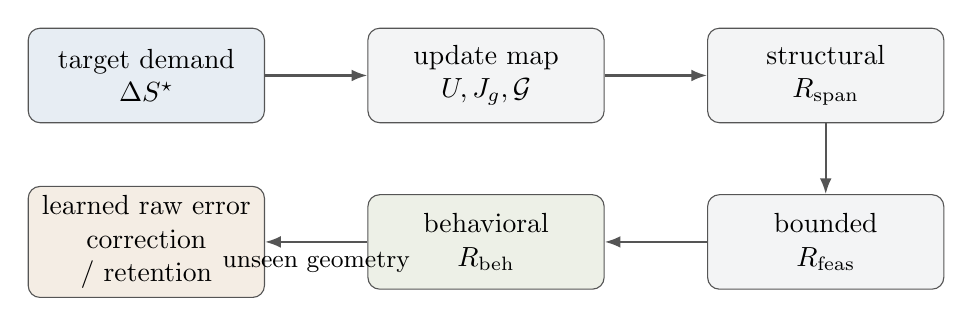
\begin{tikzpicture}[
 node distance=9mm and 13mm,
 b/.style={draw=Line,rounded corners=1.5mm,fill=Panel,minimum width=30mm,minimum height=12mm,text width=27mm,align=center},
 a/.style={-{Latex[length=2mm]},thick,draw=Line}
]
\node[b,fill=Core] (target) {target demand\\$\Delta S^\star$};
\node[b,right=of target] (map) {update map\\$U,J_g,\mathcal G$};
\node[b,right=of map] (span) {structural\\$R_{\mathrm{span}}$};
\node[b,below=of span] (feas) {bounded\\$R_{\mathrm{feas}}$};
\node[b,left=of feas,fill=Theory] (beh) {behavioral\\$R_{\mathrm{beh}}$};
\node[b,left=of beh,fill=Secondary] (error) {learned raw error\\correction / retention};
\draw[a] (target)--(map);\draw[a] (map)--(span);\draw[a] (span)--(feas);\draw[a] (feas)--(beh);\draw[a] (beh)--node[below,font=\small]{unseen geometry}(error);
\end{tikzpicture}
\caption{H1은 단순 rank가 아니라 bounded behavioral reachability를 검증한다.}
\end{figure}

\subsection{Correction과 retention}
Affected readout 집합을 $Q_{\mathrm{aff}}$, unaffected association을 $I_{\mathrm{keep}}$라 둔다.
\[
E_{\mathrm{corr}}=
\frac{1}{|Q_{\mathrm{aff}}|}
\sum_{q\in Q_{\mathrm{aff}}}
\|r_q(S')-r_q(S^\star)\|_2^2,
\]
\[
E_{\mathrm{retain}}=
\frac{1}{|I_{\mathrm{keep}}|}
\sum_{i\in I_{\mathrm{keep}}}
\|k_i^\top S'-k_i^\top S^\star\|_2^2.
\]
Affected key는 retention에서 제외한다. $\exp(-\mathrm{MSE})$ harmonic joint는 Pareto plot의 secondary metric이며 confirmatory estimand가 아니다.

\section{가설과 실험}
\begin{figure}[t]
\centering
\begin{tikzpicture}[
 node distance=7mm,
 c/.style={draw=Line,rounded corners=1.5mm,fill=Core,minimum width=147mm,minimum height=10mm,text width=140mm,align=left,inner xsep=3mm},
 s/.style={draw=Line,rounded corners=1.5mm,fill=Theory,minimum width=147mm,minimum height=10mm,text width=140mm,align=left,inner xsep=3mm},
 e/.style={draw=Line,rounded corners=1.5mm,fill=Secondary,minimum width=147mm,minimum height=10mm,text width=140mm,align=left,inner xsep=3mm},
 a/.style={-{Latex[length=2mm]},thick,draw=Line}
]
\node[c] (h1) {\textbf{H1} constrained behavioral regret가 unseen-geometry learned error를 예측하는가?};
\node[c,below=of h1] (h2) {\textbf{H2} independent erase/write가 asymmetric demand를 개선하면서 symmetric operation과 retention을 보존하는가?};
\node[c,below=of h2] (h4) {\textbf{H4} 그 이득이 relevant intervention으로 사라지고 matched rescue로 회복되는가?};
\node[s,below=of h4] (h3) {\textbf{H3 parallel} diagonal control의 충분성은 demand family의 joint diagonalizability로 결정되는가?};
\node[e,below=of h3] (h5) {\textbf{H5-lite} operation label 없이 held-out SUPERSEDE에서 같은 방향이 유지되는가?};
\draw[a] (h1)--(h2);\draw[a] (h2)--(h4);\draw[a,dashed] (h2)--(h3);\draw[a,dashed] (h4)--(h5);
\end{tikzpicture}
\caption{직렬 claim chain은 H1$\rightarrow$H2$\rightarrow$H4다. H3는 병렬 이론 branch, H5는 anchor다.}
\end{figure}

\subsection{H1: Constrained behavioral reachability}
\textbf{가설.} OracleCandidate에서 operation fixed effect를 통제한 뒤에도 $R_{\mathrm{beh}}^2$가 unseen geometry의 learned behavioral MSE를 예측한다.

\textbf{변수.} Association load, key correlation, $\|A\|/\|B\|$, old/new cosine, candidate contamination을 episode 내부에서 변화시킨다. Train과 test geometry를 분리한다.

\textbf{통계 모델.}
\[
E_{i,s}^{\mathrm{learned}}=
\alpha+\beta R_{\mathrm{beh},i}^2+
\gamma_{\operatorname{op}(i)}+u_s+\epsilon_{i,s}.
\]
Primary unseen-geometry $R^2$는 operation-only model 대비
$1-\mathrm{SSE}_{\mathrm{full}}/\mathrm{SSE}_{\mathrm{op-only}}$로 계산하여
operation identity 자체의 설명력을 제외한다. Seed exact sign-flip은 각 seed의
unseen test geometry에서 다시 추정한 operation-adjusted slope에 적용한다.
Calibration slope는 primary descriptive diagnostic으로 보고하되 사전 equivalence
margin이 없으므로 confirmatory gate에는 넣지 않는다. State-span regret와
state-feasible regret는 comparative diagnostic이다.

\textbf{판정.} OracleCandidate에서 예측력이 있어야 H1을 연다. RecurrentRead에서 추가되는 error는 candidate-recovery 및 content-interference gap으로 보고한다.

\subsection{H2: Magnitude factorization}
두 조건은 동일 two-output head $(\tilde e,\tilde w)$를 사용한다. Tied만
\[
(\tilde e,\tilde w)\mapsto(\beta,\beta),\qquad
\beta=(\tilde e+\tilde w)/2
\]
로 diagonal subspace에 projection한다.

H2는 다음을 모두 만족해야 한다.
\begin{enumerate}
\item ADD/INVALIDATE normalized absolute gain $>\delta_{\mathrm{asym}}$;
\item PRESERVE effect CI $\subset[-\delta_P,\delta_P]$;
\item SUPERSEDE relative effect CI $\subset[-\delta_S,\delta_S]$;
\item asymmetric-minus-symmetric interaction $>0$;
\item unaffected retention degradation $\le\epsilon_{\mathrm{ret}}$;
\item equal-budget validation tuning이 strict-recipe 방향을 뒤집지 않음.
\end{enumerate}

Normalized gain은 최소 headroom을 넘는 episode에서 tied-to-oracle gap 중 dual이 닫은 비율이며 SESOI는 그 gap의 사전 고정 비율이다. Headroom이 지나치게 작은 episode는 ADD/INVALIDATE와 SUPERSEDE normalized analysis에서 제외하되 raw MSE 표에는 남긴다. 8 paired training seeds를 사용한다. Episode paired bootstrap은 8개 checkpoint를 고정한 채 operation strata 내부 episode만 재표집하고, seed exact sign-flip($2^8=256$)은 별도로 계산한다.

\subsection{H3: Joint diagonalizability}
한 개의 common rotation은 representation basis로 흡수할 수 있다. 따라서 demand family 전체가 하나의 shared basis에서 동시에 diagonalizable한지가 핵심이다.
\[
\kappa=\E_{i,j}\|P_iP_j-P_jP_i\|_F,
\]
\[
R_{\mathrm{JD}}=
\min_{Q^\top Q=I}
\sum_\tau\|\operatorname{offdiag}(Q^\top P_\tau Q)\|_F^2.
\]
구현은 위 raw objective와 함께
$R_{\mathrm{JD}}/(|\mathcal{T}|d^2)$를 operator-entry MSE 단위의 normalized
regret로 보고한다. 각 seed에서 24개 operator로 shared basis를 학습하고 별도
8개 operator에서 평가한다. 또한 성분 분산이 $1/d$인 held-out isotropic probe에
operator를 적용하여 normalized regret가 실제 application MSE를 예측하는지
calibration slope와 $R^2$로 검증한다.

\begin{center}
\begin{tabular}{lll}
\toprule
Family & Shared-basis property & 예측 \\
\midrule
Axis commuting & 현재 basis에서 diagonal & fixed diagonal 충분 \\
Common-rotated commuting & 공통 $Q$에서 diagonal & learned basis가 회복 \\
Noncommuting & 공통 diagonal basis 없음 & diagonal residual, low-rank 회복 \\
\bottomrule
\end{tabular}
\end{center}

Controller는 같은 target projector를 demand descriptor로 받는다. Transaction-conditioned low-rank operator는 richer-control oracle upper bound로 명시하며, learned shared-basis diagonal과 동일한 의미의 parameter-matched model로 해석하지 않는다. Error와 active control dimension/parameter/FLOP frontier를 함께 보고한다. 네 paired contrast는 normalized regret $10^{-3}$의 사전 practical threshold와 8-seed exact sign-flip을 모두 넘어야 한다. 이와 별도로 axis fixed 및 common-rotation learned residual의 absolute near-zero, noncommuting commutator와 shared-basis residual의 positive separation, low-rank/full oracle recovery를 요구한다.

\subsection{H4: Functional mediation}
E02의 8 paired-seed checkpoint를 freeze한다. 같은 $S,A,B$에서 operation만 바꾼 counterfactual quartet을 사용한다.

\textbf{Primary.} Relevant intervention damage $-$ irrelevant intervention damage의 operation interaction.

\textbf{Support.}
\begin{itemize}
\item gate dose $0,0.25,0.5,0.75,1$의 monotonicity;
\item independent same-operation donor와 같은 $S,A,B$의 cross-operation donor를 gate norm에 맞춰 transplant;
\item relevant gate zeroing 뒤 independent same-operation 또는 oracle gate로 relevant component만 복원하는 nontrivial rescue;
\item post-hoc scalarization이 trained tied-vs-dual gap을 얼마나 재현하는지 mediation fraction으로 보고.
\end{itemize}

원래 gate를 그대로 되돌리는 것은 sanity check일 뿐 confirmatory rescue가 아니다.

\subsection{H5-lite: Semantic anchor}
Operation one-hot, oracle $(e,w)$, exact mask를 입력하지 않는다. Structured records에서 version, validity, prior/current relation을 읽는다.

\begin{center}
\begin{tabular}{ll}
\toprule
Split & 검증 대상 \\
\midrule
Held-out SUPERSEDE, seen domain/template & demand composition (primary) \\
Seen operation, held-out paraphrase & surface robustness \\
Seen operation, held-out domain & domain transfer \\
SUPERSEDE + new domain + paraphrase & combined stress \\
\bottomrule
\end{tabular}
\end{center}

Primary는 oracle address + hidden old value이며 hidden address 조건과 동시에 claim하지 않는다. 300-item audit는 split/domain stratification, two independent reviewers, agreement, adjudication을 기록한다. Meaning preservation $\ge0.95$, answer leakage $\le0.02$, reviewer agreement $\ge0.80$을 모두 만족하기 전에는 semantic claim을 열지 않는다.

\subsection{H6와 RQ-T}
H6는 multi-update, plan continuation, repeated query에서 one-time assimilation, retrieve-every-query, retrieve-once cached snapshot을 quality-constrained cost로 비교한다.
\[
m_q^\star=
\min\{m:C_{\mathrm{assim}}(m)<C_b(m),
E_{\mathrm{corr}}\le\epsilon_c,
E_{\mathrm{retain}}\le\epsilon_r\}.
\]
RQ-T는 KVEraser\citep{kveraser2026}, typed append, suffix/full re-prefill을 operation-matched로 비교하지만 official revision과 localization parity가 확보될 때까지 workshop claim에 포함하지 않는다.

\section{실험 단계와 repository 매핑}
\begin{longtable}{p{11mm}p{55mm}p{49mm}p{39mm}}
\toprule
단계 & Entry point & 산출물 & 역할 \\
\midrule
\endfirsthead
\toprule
단계 & Entry point & 산출물 & 역할 \\
\midrule
\endhead
E00 & \makecell[l]{\footnotesize\ttfamily e00\_protocol\_lock.py} & 기존 environment/protocol artifact & 실행 중 변경 금지 \\
E01 & \makecell[l]{\footnotesize\ttfamily e01\_local\_\\controllability.py} & 기존 v6.0 pilot & confirmatory 아님 \\
E01b & \makecell[l]{\footnotesize\ttfamily e01b\_constrained\_\\behavioral\_reachability.py} & per-episode regret/error, unseen calibration & H1 \\
E02 & \makecell[l]{\footnotesize\ttfamily e02\_magnitude\_\\factorization.py} & 8-seed tied/dual, raw metric, strict+tuned & H2 \\
E03 & \makecell[l]{\footnotesize\ttfamily e03\_granularity\_\\orientation.py} & commutator, JD gap, operator frontier & H3 \\
E04 & \makecell[l]{\footnotesize\ttfamily e04\_functional\_\\mediation.py} & dose/transplant/rescue & H4 \\
E05 & \makecell[l]{\footnotesize\ttfamily e05\_semantic\_demand\_\\inference.py} & OOD splits, audit CSV & H5 anchor \\
E06 & \makecell[l]{\footnotesize\ttfamily e06\_reusable\_state\_\\assimilation.py} & chain, plan, quality break-even & extension \\
E07 & \makecell[l]{\footnotesize\ttfamily e07\_transformer\_\\boundary.py} & official backend only & extension \\
E08 & \makecell[l]{\footnotesize\ttfamily e08\_claim\_freeze.py} & evidence registry, claim tiers & 필수 \\
\bottomrule
\end{longtable}

\section{현재 E00/E01 실행과 joint injection}
현재 동작 중인 E00/E01의 fingerprint를 보존하기 위해 live repository를 수정하지 않는다. 두 run은 v6.0 pilot로 끝까지 보존하고, 종료 뒤 additive patch를 적용한다.

\begin{enumerate}
\item active process가 없음을 확인한다.
\item E00/E01 import closure의 hash를 확인한다.
\item E01b와 새 theory/data/model module을 추가한다.
\item E02--E08, config, docs만 교체한다.
\item compile, pytest, config audit, CPU dry-run을 수행한다.
\item E01b부터 confirmatory evidence를 생성한다.
\end{enumerate}

Patch는 E00, E01, common runner와 해당 import closure를 한 개도 덮어쓰지 않는다.

\section{통계와 claim gate}
Episode paired bootstrap은 고정 checkpoint의 test-set uncertainty를, seed exact sign-flip은 training replicate uncertainty를 측정한다. Episode 수를 늘려 seed uncertainty를 인위적으로 줄이지 않는다.

Hierarchical gatekeeping은 다음과 같다.
\begin{enumerate}
\item H1이 통과해야 H2 claim을 연다.
\item H2가 통과해야 H4 mediation claim을 연다.
\item H3는 별도 theory branch다.
\item H5는 exploratory anchor이며 audit가 완료돼야 한다.
\item H6/RQ-T는 workshop claim ceiling을 올리지 않는다.
\end{enumerate}

\section{제출 범위와 일정}
REALM short paper의 본문은 H1--H4를 중심으로 구성하고 H5는 작은 anchor만 포함한다.

\begin{center}
\begin{tabular}{lll}
\toprule
시점 & 작업 & 종료 조건 \\
\midrule
E00/E01 종료 직후 & patch + E01b smoke & frozen hash 유지, test PASS \\
Day 1 & E01b main & OOS calibration artifact \\
Day 2--3 & E02 8 seeds & five guardrails + raw JSONL \\
Day 3--4 & E04 8 seeds & primary/support contrasts \\
Day 4 & E03 theory & JD figure/table \\
Day 5 & H5-lite & primary split + audit export \\
Day 6 & E08 freeze & claim registry fixed \\
Day 7--9 & clean rerun, paper, anonymization & submission bundle \\
\bottomrule
\end{tabular}
\end{center}

\section{결과별 허용 주장}
\begin{longtable}{p{62mm}p{87mm}}
\toprule
관찰 & 최대 허용 주장 \\
\midrule
H1만 통과 & bounded behavioral reachability가 finite-memory update error를 예측한다. \\
H1+H2 & independent erase/write magnitude가 asymmetric demand interference를 줄인다. \\
H3 & diagonal control의 충분성이 demand family의 joint diagonalizability에 의존한다. \\
H1+H2+H4 & factorization advantage가 operation-specific function으로 매개된다. \\
H5 방향+audit & structured semantic transaction의 작은 external-validity anchor. \\
DID만 양수 & H2 금지; symmetric degradation artifact 가능성. \\
Zeroing만 양성 & necessity diagnostic만 허용; mediation 금지. \\
Mock E07 & Transformer systems claim 금지. \\
\bottomrule
\end{longtable}

\section{최종 메시지와 장기 확장}
\begin{claimbox}
Finite memory의 update 실패는 gate 수 자체가 아니라, environment가 요구하는 target-update family와 controller가 실제 bounded gate set에서 제공하는 behavioral reachable geometry의 rank, orientation, conditioning이 맞지 않을 때 발생한다. CATENA v6.1은 이를 constrained regret, factorization guardrail, joint diagonalizability, counterfactual intervention으로 검증한다.
\end{claimbox}

후속 연구에서는 external state를 의미론적으로 명시적으로 유지하고 internal state는 dense하고 entangled한 채 update control만 softly addressable하게 만든다. Multimodal observation과 action-conditioned future prediction은 controlled core가 성립한 뒤 world-model 방향으로 확장한다.

\begingroup
\sloppy
\printbibliography
\endgroup
\end{document}
